\chapter{Experiments}
\section{Empirical Analysis} \label{exp}
To evaluate Polyanya OkNN we consider two distinct setups and one large map with 
containing 9000 polygonal obstacles (this benchmark is described further in the next section).

In the first setup, targets are numerous and densely distributed throughout
the map. Our principal point of comparison in this case is \textit{LVG}~\cite{zhang2004spatial} which
is a state of the art method based on incremental visibility graphs. 
In the second setup, targets are few and sparsely distributed. Our principal point of comparison in
this case is brute-force
point-to-point search with \textit{Polyanya}. As per Algorithm~\ref{brute}, we run one complete search for each candidate in the target set. We motivate these decisions as follows:

\begin{itemize}[leftmargin=1cm]
\item When the map is large and targets are many (commonly the case in spatial database settings) \textit{LVG} considers only a small part of map and so its query processing can be very fast. Brute force Polyanaya meanwhile is infeasible to run (there are too many searches).

\item When the map is large targets are few ($<$15) \textit{LVG} builds a visibility graph for almost entire map, and ends up with quadratic runtime complexity, which is unacceptable. Meanwhile, brute force \textit{Polyanya}, which is a very fast point-to-point pathfinding algorithm, can be competitive even when called repeatedly. This comparison is motivated by recent prior work involving kNN queries on road networks~\cite{abeywickrama2016k}, where other fast single-pair algorithms were shown to provide state-of-the-art performance in multi-targets scenarios, even when compared against dedicated kNN algorithms.
\end{itemize}

We implemented in C++ the LVG algorithm (more details below) as well as two versions of multi-target Polyanya: one each for Target and Interval Heuristic. Our code is compiled with \textit{clang-902.0.39.1} using \textit{-O3} flag, under \textit{x86\_64-apple-darwin17.5.0} platform. All of our source code and test data set are  publicly available \footnote{TBD}. All experiments are performed on a 2.5 GHz Intel Core i7 machine with 16GB of RAM and running OSX 10.13.4. 

\begin{algorithm}
  \input{./code/brute_polyanya.pseudo}
  \caption{Brute force Polyanya. We adapt the point-to-point algorithm for OkNN by searching once
  for each target in the candidate set.}
  \label{brute}
\end{algorithm}

\subsection{Implementation of \textit{LVG}}
As discussed \textit{LVG} is our primary competitor in experiments with dense targets. However, since there is no publicly available implementation, we write one ourselves. We implement the method as per the description in the original paper~\cite{zhang2004spatial}. The only differences is in construction of the visibility graph: \textit{LVG} uses the rotational plane-sweeping algorithm from~\cite{sharir1986shortest} which runs worst case $O(n^2logn)$ time. In our work we opted to simplify development complexity and use a \textit{R*-tree}~\cite{beckmann1990r} query for visibility checking. Each such query runs in $log(n)$ time  and we perform one check for each unique pair of vertices. Thus the total complexity to build a visibility graph is also $O(n^2logn)$. This implementation, as with the rest of our code, is made publicly available.

The implmentation of \textit{R*-tree} we use is also publicly available \footnote{https://github.com/safarisoul/ResearchProjects/tree/master/2016-ICDE-RkFN}, and appears in other recently published work~\cite{wang2016efficiently}.

\subsection{Benchmark} \label{bm}
The data set from our main competitor LVG\cite{zhang2004spatial} is no longer available on the public Internet so we opt to generate new benchmark problems.
We extract the shape of all parks in Australia from \textit{OpenStreetMap}\cite{OpenStreetMap} and
use these shapes as polygonal obstacles. There are about 9000 such polygons in total.
Next we generate a map by tiling all obstacles in the empty square plane.
For the tiling, we first divide the square plane into grid having $\textit{ceil}(\sqrt{|O|})$ number of rows and columns.
Then we assign each polygon to a single grid cell and normalize the shape of polygon by to fit inside the cell.Figure~\ref{distribution} gives an example a map generated in this way.

One thing needs to be highlighted is that, unlike \textit{LVG} ~\cite{zhang2004spatial} where obstacles are always rectangular, we consider polygons of arbitrary shape, which is more realistic and potentially more challenging as there are more vertices to consider. The total number of vertices across all polygons is more than 100,000. 

\begin{figure}[t]
  \centering
  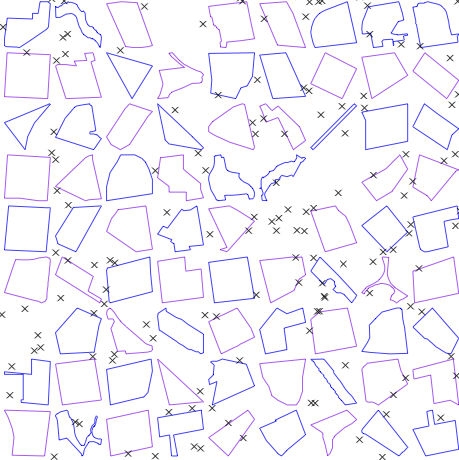
\includegraphics[width=\linewidth]{pic/distribution.png}
  \caption{Example: a generated map with many targets.}\label{distribution}
\end{figure}

\subsection{Experiment 1: lower bounds on performance}

\begin{figure*}[!htbp]
    \centering
    
    \begin{subfigure}[b]{0.5\textwidth}
        \centering
        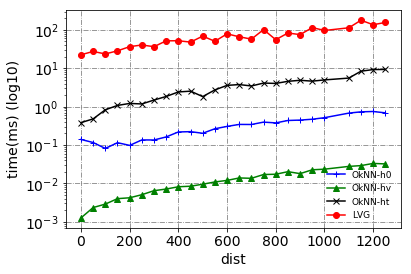
\includegraphics[width=.7\textwidth]{pic/e1_dense_time.png}
        \caption{Time \textit{vs.} $dist$}
        \label{e1_dense_time}
    \end{subfigure}%
    \hfill
    \begin{subfigure}[b]{0.5\textwidth}
        \centering
        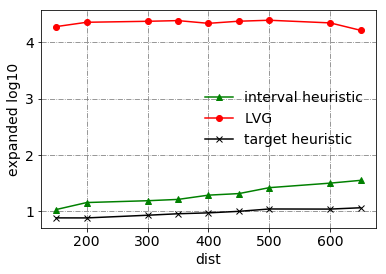
\includegraphics[width=.7\textwidth]{pic/e1_dense_gen.png}
        \caption{\small Expanded node \textit{vs.} $dist$}
        \label{e1_dense_gen}
    \end{subfigure}
    \caption{\small Experiment 1: Dense}
\end{figure*}

\begin{figure*}[!htbp]
    \centering
    \begin{subfigure}[b]{0.5\textwidth}
        \centering
        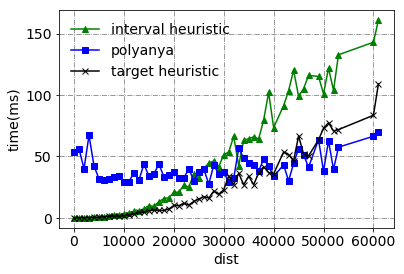
\includegraphics[width=.7\textwidth]{pic/e1_sparse_time.png}
        \caption{Time \textit{vs.} $dist$}
        \label{e1_sparse_time}
    \end{subfigure}%
    \hfill
    \begin{subfigure}[b]{0.5\textwidth}
        \centering
        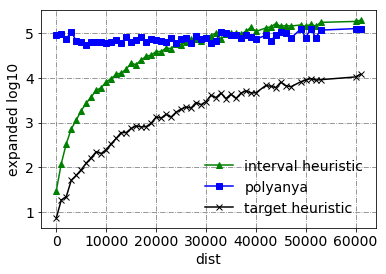
\includegraphics[width=.7\textwidth]{pic/e1_sparse_gen.png}
        \caption{\small Expanded node \textit{vs.} $dist$}
        \label{e1_sparse_gen}
    \end{subfigure}
    \caption{\small Experiment 1: Sparse}

\end{figure*}

The aim of this experiment is to examine the performance of proposed algorithms in the easiest case, which is $k=1$. Configuration parameters for the experiment are: $|O|=9000,k=1$, $|T|=|O|$ (dense) and $|T|=6$ (sparse). Results are given in

% \begin{figure}[htbp]
%     \centering
%     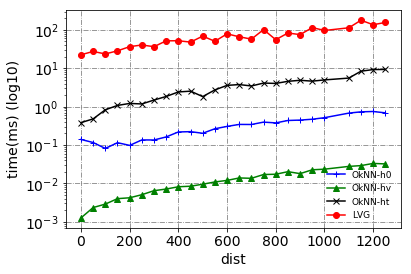
\includegraphics[width=.7\linewidth]{pic/e1_dense_time.png}
%     \caption{Dense: time \textit{vs.} $dist$}
%     \label{e1_dense_time}
% \end{figure}

% \begin{figure}[htbp]
%     \centering
%     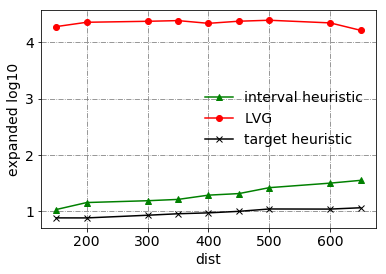
\includegraphics[width=.7\linewidth]{pic/e1_dense_gen.png}
%     \caption{Dense: expanded node \textit{vs.} $dist$}
%     \label{e1_dense_gen}
% \end{figure}

% \begin{figure}[htbp]
%     \centering
%     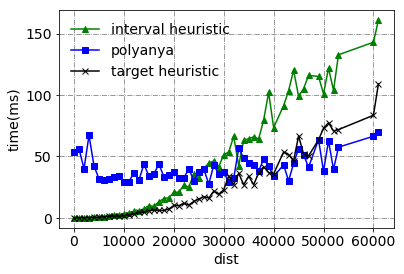
\includegraphics[width=.7\linewidth]{pic/e1_sparse_time.png}
%     \caption{Sparse: time \textit{vs.} $dist$}
%     \label{e1_sparse_time}
% \end{figure}

% \begin{figure}[htbp]
%     \centering
%     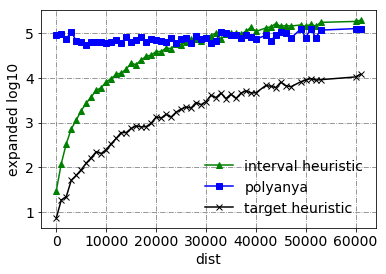
\includegraphics[width=.7\linewidth]{pic/e1_sparse_gen.png}
%     \caption{Sparse: expanded node \textit{vs.} $dist$}
%     \label{e1_sparse_gen}
% \end{figure}

Results show that in dense targets scenario, the proposed algorithms outperform \textit{LVG} in both space and time (fig~\ref{e1_dense_time},\ref{e1_dense_gen}). In the sparse targets scenario, \textit{target heuristic} has the smallest number of node operations (fig~\ref{e1_sparse_gen}), but it is outperformed on runtime by brute-force \textit{Polyanya} (fig~\ref{e1_sparse_time}) as $dist$ increases. This result suggests the algorithm has a costly heuristic function.

\subsection{Experiment 2: computing more nearest neighbor}

\begin{figure*}[!htbp]
    \centering

    \begin{subfigure}[b]{0.5\textwidth}
        \centering
        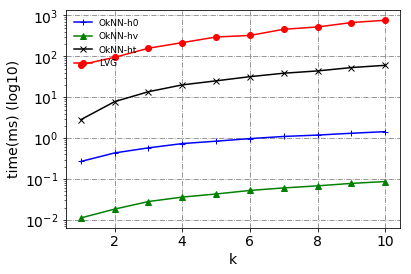
\includegraphics[width=.7\textwidth]{pic/e2_dense_time.png}
        \caption{Time \textit{vs.} $k$}
        \label{e2_dense_time}
    \end{subfigure}%
    \hfill
    \begin{subfigure}[b]{0.5\textwidth}
        \centering
        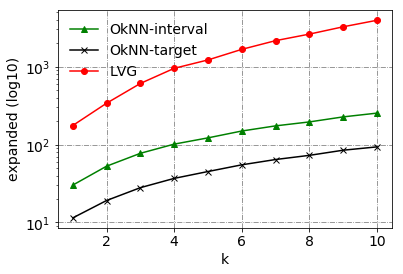
\includegraphics[width=.7\textwidth]{pic/e2_dense_gen.png}
        \caption{Expanded node \textit{vs.} $k$}
        \label{e2_dense_gen}
    \end{subfigure}
    \caption{Experiment 2: Dense}
\end{figure*}

\begin{figure*}[!htbp]
    \centering
    
    \begin{subfigure}[b]{0.5\textwidth}
        \centering
        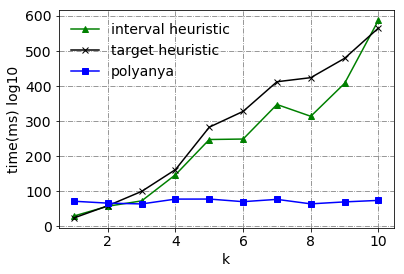
\includegraphics[width=.7\textwidth]{pic/e2_sparse_time.png}
        \caption{\small Time \textit{vs.} $k$}
        \label{e2_sparse_time}
    \end{subfigure}%
    \hfill
    \begin{subfigure}[b]{0.5\textwidth}
        \centering
        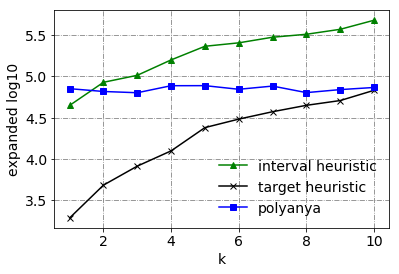
\includegraphics[width=.7\textwidth]{pic/e2_sparse_gen.png}
        \caption{\small Expanded node \textit{vs.} $k$}
        \label{e2_sparse_gen}
    \end{subfigure}
    \caption{\small Experitment 2: Sparse}
    
\end{figure*}

The aim of this experiment is to examine the performance of algorithm when query becomes harder ($k$ increasing).The configuration parameters of the experiment are: $|O|=9000,k \in [1,...10]$, $|T|=|O|$ (dense), and $|T|=10$ (sparse).

% \begin{figure}[htbp]
%     \centering
%     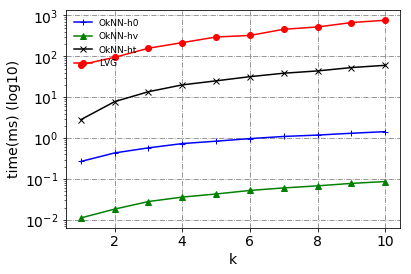
\includegraphics[width=.7\linewidth]{pic/e2_dense_time.png}
%     \caption{Dense: time \textit{vs.} $k$}
%     \label{e2_dense_time}
% \end{figure}

% \begin{figure}[htbp]
%     \centering
%     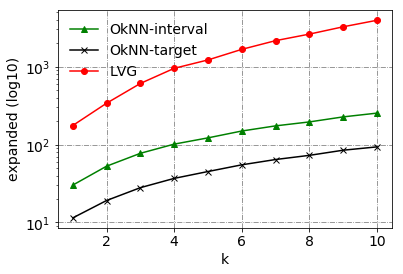
\includegraphics[width=.7\linewidth]{pic/e2_dense_gen.png}
%     \caption{Dense: expanded node \textit{vs.} $k$}
%     \label{e2_dense_gen}
% \end{figure}

% \begin{figure}[htbp]
%     \centering
%     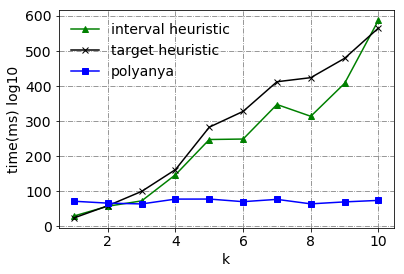
\includegraphics[width=.7\linewidth]{pic/e2_sparse_time.png}
%     \caption{Sparse: time \textit{vs.} $k$}
%     \label{e2_sparse_time}
% \end{figure}

% \begin{figure}[htbp]
%     \centering
%     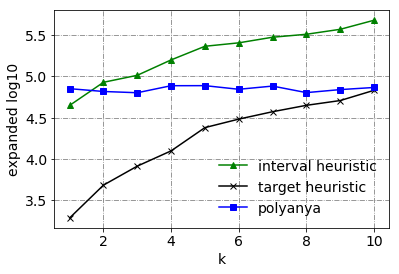
\includegraphics[width=.7\linewidth]{pic/e2_sparse_gen.png}
%     \caption{Sparse: expanded node \textit{vs.} $k$}
%     \label{e2_sparse_gen}
% \end{figure}

Results show that, in the dense targets scenario, the proposed algorithms still outcompete \textit{LVG}, even as $k$ increases (fig~\ref{e2_dense_time},\ref{e2_dense_gen}). In the sparse targets scenario we find that brute-force $Polyanya$ is not sensitive to $k$. Meanwhile each of the two OkNN variants requires increasing amounts of node operations (and thus memory) and become quickly outperformed. A side effect of \textit{target heuristic} when $k$ increase is that \textit{lazy reassign} causes extra node expansions.

\subsection{Experiment 3: changing number of targets}

\begin{figure}[!htbp]
    \centering
    \begin{subfigure}[htbp]{0.5\textwidth}
        \centering
        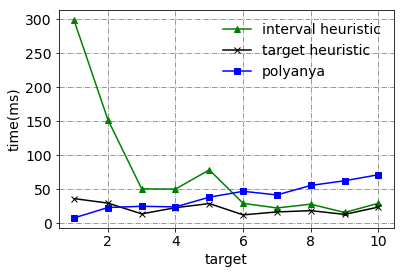
\includegraphics[width=.7\textwidth]{pic/e3_time.png}
        \caption{Time \textit{vs.} $|T|$}
        \label{e3_time}
    \end{subfigure}%
    \hfill
    \begin{subfigure}[htbp]{0.5\textwidth}
        \centering
        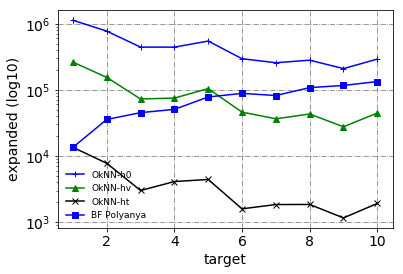
\includegraphics[width=.7\textwidth]{pic/e3_gen.png}
        \caption{Expanded \textit{vs.} $|T|$}
        \label{e3_gen}
    \end{subfigure}
    \caption{Experiment 3: Sparse}
\end{figure}

This experiment is run only on the sparse target set. The aim of this experiment is to examine the scalability of the proposed algorithms with an increasing
(but still sparse) number of targets. The configuration parameters of this experiment are: $|O|=9000,k=1,|T| \in [1,...10]$. 

% \begin{figure}[htbp]
%     \centering
%     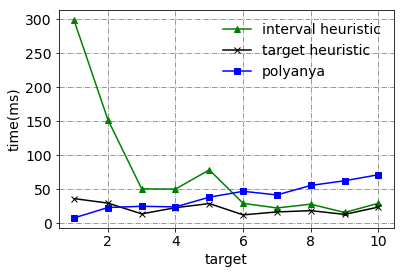
\includegraphics[width=.7\linewidth]{pic/e3_time.png}
%     \caption{Sparse: time \textit{vs.} $|T|$}
%     \label{e3_time}
% \end{figure}

% \begin{figure}[htbp]
%     \centering
%     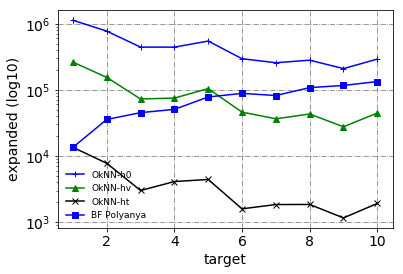
\includegraphics[width=.7\linewidth]{pic/e3_gen.png}
%     \caption{Sparse: expanded \textit{vs.} $|T|$}
%     \label{e3_gen}
% \end{figure}

Results show that proposed algorithms gradually outcompete brute force \textit{Polyanya} in both time and node operations (fig~\ref{e3_time},\ref{e3_gen}). This implies that the proposed OkNN variants algorithms are much better choices when the set of targets increase. Although we have seen in other experiements that brute-force \textit{Polyanya} has an advantage when $k$ is large, this advantaged disappears as $|T|$ grows. In some practical settings $|T|$ can be in the hundreds or thousands, e.g.~\cite{abeywickrama2016k} while $k$ is usually orders of magnitude smaller. 


